\section{方差比较的条件}
\label{sec:vr-comparison}

说一种方法“方差更小”之前，先要讲清楚和什么比、在什么预算下比。一种方法每个样本的方差只有原来的一半，但每个样本的计算时间是原来的三倍，它在同样的时间内得到的结果反而更差。另一种方法方差很小，却有偏差，单看方差会高估它。本节规定全章比较估计量的口径。

\paragraph{基准}
前两章把目标分布记作$\pi$；本章常要同时处理目标与另一个抽样分布的密度，因此把目标分布记作$P$，密度记作$p$。

固定样本空间$\mathcal{X}$上的概率分布$P$与函数$f$，设$f$在$P$下可积，待算的积分是
\[
 I=\mathbb{E}_P[f(X)] .
\]
基准是第~\ref{chap:monte-carlo-integration-error}章的独立样本平均：$X_1,\dots,X_n$独立且都服从$P$，
\[
 \hat{I}_n=\frac1n\sum_{i=1}^{n}f(X_i) .
\]
估计$\hat{I}_n$无偏；若再有$\mathbb{E}_P[f(X)^2]<\infty$，记$\sigma^2=\operatorname{Var}_P(f(X))$，则$\operatorname{Var}(\hat{I}_n)=\sigma^2/n$。本章的方法都在这一基准上改动，并且大多保留一个结构：估计量由若干个相互独立的“单元”平均而成。单元可以是一个样本，也可以是一对样本、一组分层样本或一个随机化点集。

\paragraph{方差乘成本}
设一个单元输出随机变量$Y$，满足$\mathbb{E}[Y]=I$与$v=\operatorname{Var}(Y)<\infty$，生成一个单元的平均成本为$c>0$。成本按实际计算计入：生成基础随机数、把它变换成样本、求$f$的值，以及权重、辅助函数、密度等额外计算。总预算为$C$时可以算$m=C/c$个独立单元（暂不计取整），平均值的方差为
\begin{equation}
 \operatorname{Var}\Bigl(\frac1m\sum_{k=1}^{m}Y_k\Bigr)=\frac{v}{m}=\frac{v\,c}{C} .
 \label{eq:vr-work-variance}
\end{equation}
预算固定时，决定精度的是乘积$v\,c$，而不是$v$本身。两种无偏方法A与B相比，定义B相对于A的\term{相对效率}（relative efficiency）为
\begin{equation}
 \operatorname{eff}(\mathrm{B}:\mathrm{A})=\frac{v_{\mathrm{A}}\,c_{\mathrm{A}}}{v_{\mathrm{B}}\,c_{\mathrm{B}}} .
 \label{eq:vr-relative-efficiency}
\end{equation}
它的含义是：要达到同样的方差，A所需的预算是B的$\operatorname{eff}(\mathrm{B}:\mathrm{A})$倍。

\paragraph{预备成本}
有些方法在正式计算前要做一次准备，例如试运行、拟合一个分布或估计一个系数。若准备的成本是固定的$C_0$，正式计算只剩$C-C_0$，式~\eqref{eq:vr-work-variance}成为$v\,c/(C-C_0)$。于是预算较小时准备可能得不偿失，预算较大时它的分摊成本才变得可以忽略。

\paragraph{尾概率的例子}
回到导言的$I=\mathbb{P}(X>4)$。直接平均记为方法A，第~\ref{sec:vr-change-distribution}节改从另一个分布抽样并乘以权重的方法记为B，在那里会算出B的单样本方差。两种方法的参数为
\[
 v_{\mathrm{A}}=0.01798,\quad c_{\mathrm{A}}=1;\qquad v_{\mathrm{B}}=0.001749,\quad c_{\mathrm{B}}=1.5 .
\]
其中$v_{\mathrm{A}}=I(1-I)$，$c_{\mathrm{B}}=1.5$假设求权重使单样本成本增加一半；另设选择抽样分布的试运行花费$C_0=2000$。不计准备时，
\[
 \operatorname{eff}(\mathrm{B}:\mathrm{A})=\frac{0.01798\times1}{0.001749\times1.5}\approx6.9 .
\]
计入准备时，两者方差相等的预算由下式确定：
\[
 \frac{0.01798}{C}=\frac{0.001749\times1.5}{C-2000} .
\]
解得$C\approx2342$。图~\ref{fig:vr-budget-crossover}画出两种方法的相对均方根误差随预算的变化：预算低于交点时，准备几乎吃掉全部预算，新方法更差；预算到$10^{5}$时，直接平均的相对误差约为$2.3\%$，新方法约为$0.89\%$。

\begin{BookInlineFigure}
 \centering
 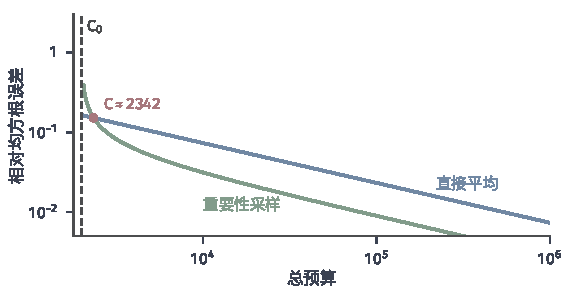
\includegraphics[width=96mm]{figures/07-probability/08-sampling-and-integration/matplotlib/vr-budget-crossover/figure.pdf}
 \caption{$I=\mathbb{P}(X>4)$，$X\sim\operatorname{Exp}(1)$，相对均方根误差$\sqrt{v\,c/(C-C_0)}/I$随总预算$C$的变化，双对数坐标。蓝线为直接平均（$v=0.01798$，$c=1$，$C_0=0$），绿线为第~\ref{sec:vr-change-distribution}节的加权估计（$v=0.001749$，$c=1.5$，$C_0=2000$），虚线标出$C_0$，红点为两者相等的预算。}
 \label{fig:vr-budget-crossover}
\end{BookInlineFigure}

\paragraph{二阶矩要逐项核对}
式~\eqref{eq:vr-work-variance}要求$v<\infty$。本章的每一种改动都会改变单元的形式：乘以权重、减去辅助量、换成条件平均或成对平均。原积分存在只说明$\mathbb{E}[\lvert Y\rvert]<\infty$，不说明$\mathbb{E}[Y^2]<\infty$。方差为无穷时，式~\eqref{eq:vr-relative-efficiency}失去意义，误差也不再按$m^{-1/2}$缩小。所以每引入一种估计量，都要单独检查它的二阶矩。

\paragraph{有偏的估计}
有些估计量不是无偏的，例如用同一批样本估计系数再代回，或者用两个平均值的比值作估计。这时比较的对象是均方误差，由第~\ref{chap:monte-carlo-integration-error}章，
\[
 \mathbb{E}\bigl[(\hat{I}-I)^2\bigr]=\bigl(\mathbb{E}[\hat{I}]-I\bigr)^2+\operatorname{Var}(\hat{I}) .
\]
常见的情形是偏差与$1/n$同阶而方差与$1/n$同阶，偏差的平方是$1/n^2$阶，样本量大时可以忽略。但样本量小时两者可能相当。另一个陷阱是：把内部样本量固定的有偏估计独立重复$R$次再平均，方差按$1/R$缩小，偏差却原样保留。这类估计的偏差要按内部样本量单独分析。

\paragraph{三个改动的位置}
一次随机计算可以看成一条流水线：基础随机数$\bm{U}$经生成映射$T$变成样本$X=T(\bm{U})$，求值得到$f(X)$，再取平均。图~\ref{fig:vr-three-routes}标出本章三类方法改动的位置。改变分布作用在生成这一步，样本改从别的分布抽取；改变计算公式作用在求值这一步，被平均的量不再是$f(X)$；改变抽样机制作用在基础随机数上，改变的是各个$\bm{U}$之间的安排。三类改动可以组合，组合后要按本节的口径重新检查期望、二阶矩和成本；在实际预算下怎样分配试运行与正式计算、怎样在方法之间取舍，由第~\ref{chap:sampling-budget-method-selection}章统一讨论。

\begin{BookInlineFigure}
 \centering
 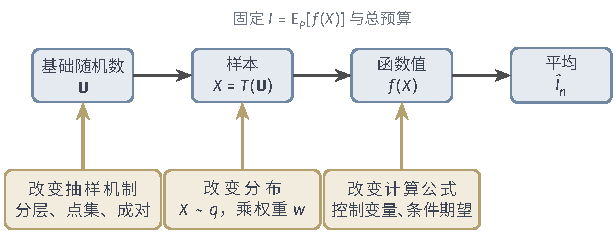
\includegraphics[width=104mm]{figures/07-probability/08-sampling-and-integration/tikz/vr-three-routes/figure.pdf}
 \caption{一次随机计算的流水线与三类方差控制方法的作用位置。上排是基础随机数、样本、函数值与平均；下排黄色框分别改动基础随机数的安排、样本的分布与被平均的量。积分$I$与总预算在比较中保持不变。}
 \label{fig:vr-three-routes}
\end{BookInlineFigure}
